\chapter{How To Qualify A Good Company To Invest In}

This chapter follows the School of Hard Knocks interview as a compact lesson in early-stage investment judgment. The transcript does not give us a valuation model or a formal underwriting formula. It gives us something more basic: a sequence of filters. We first locate the investor's mandate, then the company's stage, then the qualities that make the company worth examining, and finally the kind of help the investor expects to provide after the check is written.

\section{The Live Question}

The opening question is the chapter's problem: what do we look for in a company that we really want to invest in? That question should not be flattened into a generic checklist. The force of it is that the company is young, the evidence is incomplete, and the investor must still decide what matters.

For a candidate company \(X\), the interview's reasoning can be written as a map from a company to a small collection of early signals:
\begin{equation}
X
\longmapsto
\left(
\text{idea},
\text{team},
\text{market},
\text{stage},
\text{needed help}
\right).
\end{equation}
This is not a scoring formula from the speaker. It is a compact way to preserve the spoken order. We do not begin with a single magic number; we begin by asking whether the company belongs in the investor's actual arena.

\subsection{Question \& Answer}

\paragraph{Question.}
What are some things that we look for in a company that we really want to invest in?

\paragraph{Answer.}
We begin with context. The investment group has about \( \$50\,\mathrm{M} \) to invest, is considered venture, and works in very early rounds. Within that frame, the speaker looks for interesting ideas, thoughtful management teams, and large target markets. He then gives the scale of the bet: most investments are somewhere between about \( \$0.5\,\mathrm{M} \) and perhaps \( \$2\,\mathrm{M} \) or \( \$3\,\mathrm{M} \), in companies probably generating less than \( \$2\,\mathrm{M} \) in revenue. After that, the work turns operational: organize the company, help it hire talent, and keep the young CEO focused on what matters.

\section{Mandate And Stage}

The first move is not criteria. It is mandate. The speaker identifies a group with about
\begin{equation}
F \approx \$50\,\mathrm{M}
\end{equation}
to invest. That number matters because it defines the scale of the game. A group of this size is not buying tiny public-market positions, and it is not acting like a late-stage fund that needs enormous checks to move its own results.

The next move is categorical: the group is considered venture, and it works in very early rounds. In notation, the investment setting is roughly
\begin{equation}
\mathcal{M}
=
\left(
F \approx \$50\,\mathrm{M},
\text{venture},
\text{very early rounds}
\right).
\end{equation}
Here \(\mathcal{M}\) means mandate. It is useful because it reminds us that the later criteria are stage-specific. In a mature company, the clean financial record may carry much of the argument. In an early company, the evidence is still forming, so judgment has to include the idea, the people, and the size of the possible market.

\section{The Three-Part Screen}

Once the mandate and stage are clear, the screen appears in three parts. The speaker looks for really interesting ideas, really thoughtful management teams, and large target markets. We can keep those together as an ordered screen:
\begin{align}
\mathcal{S}(X)
&=
\bigl(
\text{interesting idea}, \nonumber\\
&\qquad
\text{thoughtful management team}, \nonumber\\
&\qquad
\text{large target market}
\bigr).
\end{align}
The order is important. The idea comes first because, at this stage, the company may not yet have enough operating history for the numbers to settle the case. But an idea alone is thin. The management team comes next because execution will determine whether the idea can survive contact with customers, hiring, and capital constraints.

The market is the third part of the same thought. Venture investing needs room. A small market may still support a fine business, but the speaker is describing venture-style investing in very early rounds. The possible market must be large enough to justify the uncertainty of acting early.

\section{Check Size And Revenue Stage}

After the qualitative screen, the speaker gives numerical discipline. Most investments are somewhere between half a million dollars and maybe two or three million dollars:
\begin{equation}
C
\approx
\$0.5\,\mathrm{M}
\quad \text{to} \quad
\$2\,\mathrm{M}\text{--}\$3\,\mathrm{M}.
\end{equation}
The upper end is intentionally approximate. The phrase ``maybe two or three million dollars'' should not be hardened into a precise ceiling. It tells us the order of magnitude of the check.

The revenue stage is also approximate:
\begin{equation}
R \lesssim \$2\,\mathrm{M}.
\end{equation}
The companies are probably generating less than \( \$2\,\mathrm{M} \) in revenue. That means they are not merely ideas, but they are also not mature machines. They are operating businesses with limited proof, limited staff, and unresolved organizational demands.

A compact stage-fit summary is therefore
\begin{align}
\text{stage fit}(X)
&\Longleftrightarrow
\left[
C_X \text{ is on the order of } \$0.5\,\mathrm{M}
\text{ to }
\$2\,\mathrm{M}\text{--}\$3\,\mathrm{M}
\right] \nonumber\\
&\qquad\qquad
\text{and}
\left[
R_X \lesssim \$2\,\mathrm{M}
\right].
\end{align}
This is not a valuation theorem. It is a careful reconstruction of the spoken boundaries: the company is early enough to need venture judgment, but real enough that revenue and hiring have already begun to matter.

\subsection{A Small Numerical Check}

Suppose, only as an example, that a candidate company has
\begin{equation}
R_X = \$1.4\,\mathrm{M},
\qquad
C_X = \$1.0\,\mathrm{M}.
\end{equation}
Then it fits the numerical neighborhood described in the interview:
\begin{align}
R_X &= \$1.4\,\mathrm{M} < \$2\,\mathrm{M},\\
C_X &= \$1.0\,\mathrm{M}
\quad \text{lies within the spoken check-size range.}
\end{align}
That is not enough to make the company investable. It only tells us that the company is in the right stage for this investor's question. We still have to return to \(\mathcal{S}(X)\): the idea, the team, and the market.

\section{From Investment To Help}

The final movement of the answer is operational. The speaker does not stop with choosing companies. After investing, the group helps focus the companies, get them organized, hire strong talent, and stay focused on the important things.

We can summarize that support mechanism as
\begin{align}
\mathcal{H}(X)
&=
\bigl(
\text{organization}, \nonumber\\
&\qquad
\text{talent}, \nonumber\\
&\qquad
\text{focus}
\bigr).
\end{align}
The reason is stated plainly: a young entrepreneur or CEO has many things coming at once and few people to deal with them. The bottleneck is not only capital. It is attention under scarcity.

So the practical update after investment is
\begin{equation}
\text{capital placed}
\quad \longrightarrow \quad
\text{organization} + \text{talent} + \text{focus}.
\end{equation}
This is the operating mechanism behind the check. The investor is not simply buying a claim about the future. The investor is trying to help the young company become coherent enough to reach that future.

\section{The Sequence As A Narrow Diagram}

The interview's logic is best kept vertical: mandate, stage, screen, check size, revenue stage, and then help. The following figure is a transcript-derived reconstruction of that order, designed as a narrow diagram for pocket-size layout.

\begin{figure}
\centering
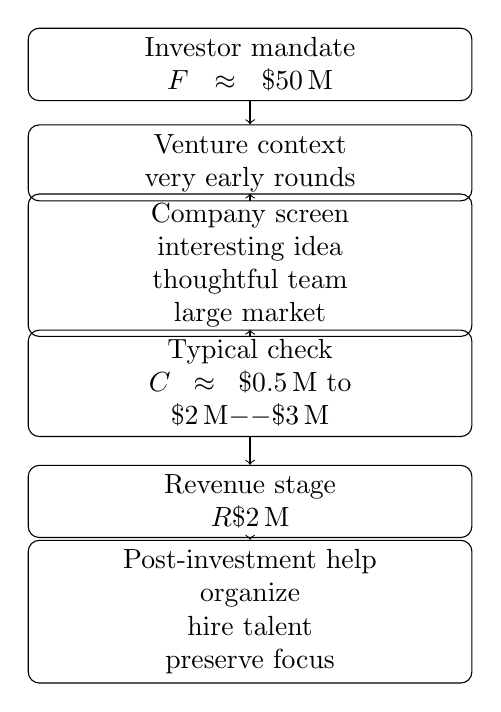
\begin{tikzpicture}[x=1cm,y=1cm]
\node[draw, rounded corners, align=center, text width=5.4cm, minimum height=0.78cm] (a) at (0,0) {Investor mandate\\ \(F \approx \$50\,\mathrm{M}\)};
\node[draw, rounded corners, align=center, text width=5.4cm, minimum height=0.78cm] (b) at (0,-1.25) {Venture context\\ very early rounds};
\node[draw, rounded corners, align=center, text width=5.4cm, minimum height=0.92cm] (c) at (0,-2.55) {Company screen\\ interesting idea\\ thoughtful team\\ large market};
\node[draw, rounded corners, align=center, text width=5.4cm, minimum height=0.78cm] (d) at (0,-4.05) {Typical check\\ \(C \approx \$0.5\,\mathrm{M}\) to\\ \(\$2\,\mathrm{M}\text{--}\$3\,\mathrm{M}\)};
\node[draw, rounded corners, align=center, text width=5.4cm, minimum height=0.78cm] (e) at (0,-5.55) {Revenue stage\\ \(R \lesssim \$2\,\mathrm{M}\)};
\node[draw, rounded corners, align=center, text width=5.4cm, minimum height=0.92cm] (f) at (0,-6.95) {Post-investment help\\ organize\\ hire talent\\ preserve focus};

\draw[->] (a.south) -- (b.north);
\draw[->] (b.south) -- (c.north);
\draw[->] (c.south) -- (d.north);
\draw[->] (d.south) -- (e.north);
\draw[->] (e.south) -- (f.north);
\end{tikzpicture}
\caption{A compact reconstruction of the spoken investment sequence: first mandate, then stage, then screen, then check size and revenue stage, and finally operating support.}
\end{figure}

\section{Summary}

The chapter's investment logic is deliberately modest. The speaker does not claim that a young company can be qualified by one equation. He gives a staged judgment. First locate the investor: about \( \$50\,\mathrm{M} \) to invest, venture-oriented, and active in very early rounds. Then locate the company: an interesting idea, a thoughtful management team, a large target market, a typical check size around \( \$0.5\,\mathrm{M} \) to \( \$2\,\mathrm{M}\text{--}\$3\,\mathrm{M} \), and revenue probably below \( \$2\,\mathrm{M} \).

The closing point is that investment and assistance belong together. The company is young enough that the CEO may not know what matters most amid all the incoming demands. The investor's role, as described here, is to choose companies with the right raw material and then help them organize, hire, and focus.